\documentclass[runningheads,a4paper]{llncs}

\usepackage{amssymb}
\setcounter{tocdepth}{3}
\usepackage[utf8]{inputenc}
\usepackage[hyphens]{url}
\usepackage{graphicx}
\usepackage{hyperref}
\usepackage{float}
\usepackage{eurosym}
\usepackage[normalem]{ulem}
\usepackage{alltt}
\usepackage{subfig}

% todo macro
\usepackage{color}
\newcommand{\todo}[1]{\noindent\textcolor{red}{{\bf \{ToDo}#1{\bf \}}}}

\newenvironment{code}[1]
{\begin{lrbox}{\inverbatim}\begin{minipage}{12cm}\begin{alltt}{#1}}
{\end{alltt}\end{minipage}\end{lrbox}\colorbox{lightgray}{\usebox{\inverbatim}}}

\newsavebox{\inverbatim}
\definecolor{lightgray}{rgb}{0.88,0.88,0.88}

\newcommand{\keywords}[1]{\par\addvspace\baselineskip
\noindent\keywordname\enspace\ignorespaces#1}

\begin{document}

\mainmatter  % start of an individual contribution

% first the title is needed
\title{Enriching Unstructured Media Content\\ About Events to Enable Semi-Automated Summaries, Compilations, and Improved\\ Search by Leveraging Social Networks}

% a short form should be given in case it is too long for the running head
\titlerunning{Enriching Unstructured Media Content}

\author{Thomas Steiner%
\thanks{Thomas Steiner is partly funded by the European Commission under Grant No. 248296 for the FP7 I-SEARCH project.}}
%
\authorrunning{Enriching Unstructured Media Content}
% (feature abused for this document to repeat the title also on left hand pages)

% the affiliations are given next; don't give your e-mail address
% unless you accept that it will be published
\institute{Universitat Politècnica de Catalunya\\
Department LSI\\
08034 Barcelona, Spain\\
\url{tsteiner@lsi.upc.edu}\\--\\ Supervised by:\\ Joaquim Gabarr\'{o} Vall\'{e}s (UPC)\\Michael Hausenblas (DERI)}

%
% NB: a more complex sample for affiliations and the mapping to the
% corresponding authors can be found in the file "llncs.dem"
% (search for the string "\mainmatter" where a contribution starts).
% "llncs.dem" accompanies the document class "llncs.cls".
%
\maketitle
\begin{abstract}
Mobile devices like smartphones together with social networks enable people to generate, share, and consume enormous amounts of media content. Common search operations, for example searching for a music clip based on artist name and song title on video platforms such as YouTube, can be achieved both based on potentially shallow human-generated metadata, or based on more profound content analysis driven by Optical Character Recognition (OCR) or Automatic Speech Recognition (ASR). However, more advanced use cases, such as summaries or compilations of several pieces of media content covering a certain event, are hard, if not impossible to fulfill at large scale. One example of such event can be a keynote speech held at a conference, where, given a stable network connection, media content is published on social networks while the event is still going on.
\keywords{Semantic Web, Linked Data, Multimedia Semantics, Social Networks, Social Semantic Web}
\end{abstract}

\section{Introduction}
In our thesis, we develop a framework for media content processing, leveraging social networks, utilizing the Web of Data, and fine-grained media content addressing schemes like Media Fragments URIs to provide a scalable and sophisticated solution to realize the above use cases. We evaluate our approach on the entity level against social media platform APIs in conjunction with Linked (Open) Data sources, comparing the current manual approaches against our semi-automated approach. Our proposed framework can be used as an extension for existing video platforms.

Official statistics~\cite{youtube:stats} from YouTube, one of the biggest online video platforms, state that more than 13 million hours of video were uploaded during 2010, and 35 hours of video are uploaded every minute. The mostly text-based video search engine behind YouTube works mainly based on textual descriptions, video titles, or user tags, but does not take semantics into account: it does not get the meaning of a video, for example whether a video tagged with ``obama" is about \textit{the} Obama, or about a person that just happens to have the same name. We speak of the semantic gap in this context. In~\cite{Smeulders}, Smeulders et al. define the semantic gap as
\begin{quotation}
\noindent ``The semantic gap is the lack of coincidence between the information that one can extract from the visual data and the interpretation that the same data have for a user in a given situation."
\end{quotation}

The remainder of this paper is structured as follows: \todo{Add structure of the paper}.

\section{Related Work}
MPEG-7~\cite{mpeg7} is a multimedia content description standard. Its formal name is Multimedia Content Description Interface. Unlike MPEG-1, -2, and -4, MPEG-7 does not deal with the actual encoding of moving pictures and audio, but rather stores metadata in XML format in order to describe multimedia content. MPEG-7 is meant to complement the previous MPEG standards, however, can also be used on its own independently. In a critical view of MPEG-7 in~\cite{Hau07}, Hausenblas et al. point out that due to the wide application the semantics of the description tools are often very general. Several works have already pointed out the lack of formal semantics of the standard that could extend the traditional text descriptions into machine understandable ones. In~\cite{Celma2007}, Celma et al. detail the problem with metadata interoperability in MPEG-7, mainly due to the lack of precise semantics. The authors explain that semantically identical metadata can be represented in multiple ways, for example using the free text tag, or using the keyword tag. Efforts~\cite{garca_semantic_2005-1} have been made to translate MPEG-7 into an ontology and through appropriate frameworks to enable its integration with other ontologies, thus enhancing interoperability, however, these efforts did not gain the traction their authors had hoped for.

The W3C Ontology for Media Resources~\cite{mediaontology} defines a set of mappings for many existing metadata formats. It aims to foster the interoperability among various kinds of metadata formats currently used to describe media resources on the Web. Using the Ontology for Media Resources, time based semantic annotations are possible using the \texttt{relation} property by linking to an RDF file or named graph containing annotations for a media resource (or fragment). Currently there is no solution for embedding a set of RDF triples directly into one of the properties of the Ontology for Media Resources.

\section{Proposed Approach}
Our objective for this thesis is to create a framework that allows for the semi-automatic generation of summaries or compilations of several pieces of media content covering a certain event and leveraging social networks. The term ``event" is defined\footnote{\url{http://wordnetweb.princeton.edu/perl/webwn?s=event}} by WordNet as ``something that happens at a given place and time". The process of generating a summary or compilation for an event includes the following proposed steps:

\begin{description}
\item [Event-Selection:] Decide on an event that shall be summarized.
\item [Micropost-Annotation:] Find relevant microposts on social networks containing links to media content about the event, and annotate the microposts one by one using RDF, leveraging data from the LOD cloud.
\item [Media-Content-Annotation:] Retrieve the pieces of media content and the accompanying metadata one by one, and annotate them using RDF, leveraging data from the LOD cloud.
\item [Media-Content-Ranking:] Rank and order the pieces of media content by relevance, creation time, duration, and other criteria.
\item [Media-Content-Compilation:] Based on the ranking, suggest a summary or compilation taking into account user constraints such as desired duration, composition (videos only, images only, combination of both), etc.
\end{description}

\section{Evaluation}
In the following we introduce our evaluation plan and present already existing evaluation for each of these steps.

\subsubsection{Event-Selection}
For this task we currently have preliminary results only. We have selected two recent events, the Semantic Technology Conference 2011 (SemTech) and the Apple Worldwide Developers Conference 2011 (WWDC), both located in San Francisco. For WWDC there is a DBpedia page (\url{db:Apple_Worldwide_Developers_Conference}), for SemTech there is just the generic event landing page (\url{http://semtech2011.semanticweb.com/}). We have disambiguated both event names with their locations using an API from previous work~\cite{twittertrends},~\cite{semwebvid}. For WWDC the plaintext labels of the named entities are ``Apple", ``San Francisco", ``Apple Inc.", ``iPhone OS", and ``Apple Worldwide Developers Conference". Each named entity is uniquely identified by a URI in the LOD cloud, which allows for ambiguity-free exploration of related entities. This is very important for the discovery of microposts on social networks in the task \emph{Micropost-Annotation} that might have links to media content, especially in cases where no unique event hashtag is known.

\subsubsection{Micropost-Annotation}
We have implemented a generic framework for the on-the-fly enrichment of social network microposts~\cite{twittertrends}. This framework has been successfully tested on overall 92 seven-day active users (as of June 22, 2011). The context of the tests was the detection of news trends in microposts, however, the general contribution of this framework is the extraction and disambiguation of named entities from microposts. Figure~\ref{fig:overtime-edge-a} shows an example. By using Google Analytics, named entity occurrences can be easily tracked over time. As an example, Figure~\ref{fig:overtime-edge-b} shows the occurrences graph generated by Analytics of the named entity ``tsunami". Japan was hit by an earthquake followed by a tsunami on March 11, exactly where the peak is on the graph. In general the occurrences graphs also for other examples indeed correspond to what we would expect from the news headlines of the considered days.

\begin{figure}[htb!]
  \begin{center}
\subfloat[Screenshot of a tweet, and a thereof extracted named entity ``gmail" with its representing DBpedia URI.]{\label{fig:overtime-edge-a}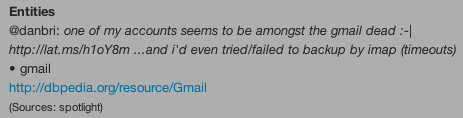
\includegraphics[width=0.46\textwidth]{./resources/twitter-swarm-nlp-tweet.png}}
\hspace{5pt}
\subfloat[Popularity of the named entity ``tsunami" from March 10 - 14. Japan was hit by a tsunami on March 11, at the peak.]{\label{fig:overtime-edge-b}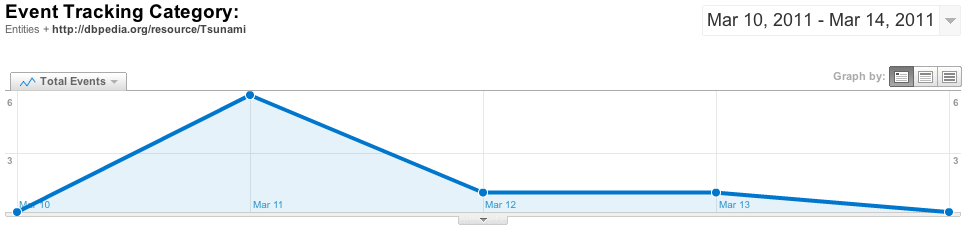
\includegraphics[width=0.47\textwidth]{./resources/twitter-swarm-nlp-tsunami.png}}
  \caption{Tweet annotation and popularity of a named entity over time.}
  \label{fig:overtime}
  \end{center}  
\end{figure}

\subsubsection{Media-Content-Annotation}
For this task we currently have preliminary results only. At present we have implemented an interactive Ajax application called SemWebVid~\cite{semwebvid} that allows for the automatic annotation of videos on YouTube with RDF. Based on the same API that powers SemWebVid, we have implemented a command line version of the annotation mechanism that in the future can be used to batch-process videos. For now, we have annotated videos with the interactive Ajax application, and reviewed the annotations manually, however, at this point, have not yet compared the annotations to a gold standard. We use the Common Tag~\cite{CommonTag:Spec} vocabulary to annotate entities in a temporal video fragment. An example can be seen in Figure~\ref{code:ctag}. This simple and consistent annotation scheme will make the comparison with a gold standard easier. Using Common Tag, both the video per se, as well as video fragments of the whole video can be annotated in the same way.

\begin{figure}[htbp!]
\begin{center}
{\footnotesize
\begin{code}
<http://www. youtube.com/watch?v=hzFp3rovfY0#t=171,177>
  a ma:MediaFragment ;
  ctag:tagged
    [ a ctag:Tag ;
      ctag:label "Commodore 64" ;
      ctag:means <http://dbpedia.org/resource/Commodore_64>
    ] .
\end{code}}
  \caption[Annotated named entity in a video fragment.]{Annotated named entity in a video fragment.}
  \label{code:ctag} 
  \end{center}  
\end{figure}

\paragraph{Whole Video Annotation}
From our experiences so far, video annotation of the whole video works accurately. Both the overall video genre tags as well as the whole video tags are adequate. We have tested with keynote and conference session videos (for examples from the Google I/O events in 2010 and 2011), political speeches (for example Barack Obama's inauguration address), but also more underground video productions such as a video\footnote{\url{http://www.youtube.com/watch?v=hzFp3rovfY0}} about the music artist Timbaland being accused of stealing a music tune from the Commodore 64 scene.

\paragraph{In-Video Annotation}
In-video annotation, i.e. tagging of video fragments, is currently still sparse in most test cases. We found that sending smaller input texts increases the recall of the NLP Web services without lowering the precision, whereas sending large input texts dramatically decreases the recall. In consequence we are considering splitting up the to-be-analyzed data into smaller pieces, at the cost of processing time and more HTTP round-trips. We found the sweet spot between recall, precision, and processing cost to be around 300 characters. This figure was also publicly confirmed by Andra\v{z} Tori, CTO of Zemanta, at his keynote speech~\cite{andraz} at the Extended Semantic Web Conference.

\subsubsection{Media-Content-Ranking}
We have no results yet for this task. We plan to let the user tweak the ranking criteria interactively, and see the effect on the ranking immediately. This could happen via sliders, where a user could change the weights of criteria like view count, duration, recency, etc. The evaluation will happen based on user feedback from a test group. We will have to test whether video genre-specific weights have to be introduced, or whether common weights across all genres reveal satisfactory results.

\subsubsection{Media-Content-Compilation}
We have no results yet for this task. Similar to the previous task \emph{Media-Content-Ranking}, we plan to let the user adjust media composition criteria on-the-fly. For the desired duration, a slider seems adequate, however, we have to do some experiments whether the video compilation can work fast enough to make the slider's reaction seem interactive. The same speed constraint applies to the video composition selection (videos only, images only, combination of both).

Obviously the quality of the final video summaries needs to be evaluated by a test group, ideally against a gold standard of human-generated \emph{event x in n seconds} videos. A typical example is the YouTube \url{http://www.youtube.com/watch?v=skrz1JsxnKc}, which has a 60 seconds summary of Steve Jobs' keynote at WWDC. The problem, however, with these user-generated summaries is that they usually use official professionally produced video footage, and not user-generated content. This allows for high quality audio and video quality, whereas user-generated content from mobile devices typically suffers from problems like noisy environments when recorded from the middle of an audience, overexposure when recorded against stage lighting, or a lack of detail when recorded from too far away. We will see in how far this is an issue once we have a working prototype of the whole framework.

\section{Future Work}
We present future work for each of the previously introduced steps.

\subsubsection{Event-Selection}
We will keep an eye on a wide variety of events, such as concerts, conferences, political demonstrations, elections, speeches, natural disasters, festivities, but also non-publicly announced events such as private parties, always given there is enough social media coverage and media content available. We will archive social network communication produced around these events for further analysis.

\subsubsection{Micropost-Annotation}
So far we have implemented a solid framework capable of annotating microposts. Future work in this task will be to further increase recall and precision by incorporating more Natural Language Processing engines both for English and non-English languages. While English is covered quite well by the existing engines, other target languages such as the so-called FIGS languages (French, Italian, German, Spanish) are still not optimally covered. Our work here will focus on the integration and the alignment of the output formats of the various NLP services, both commercial, and non-commercial. The main constraint here will be the processing time, and depending on the event the sheer amount of potentially available microposts within a short period of time (compare nation-wide elections with a private party). We will also work on improving entity consolidation and ranking algorithms when different NLP services have agreeing or contradicting results for the same input text.

\subsubsection{Media-Content-Annotation}
At present we have implemented both a command line and an interactive version of the media content annotation mechanism tailored to the YouTube video platform. Future work in this task will be to improve precision and recall by the same improvement steps as in the \emph{Micropost-Annotation} task. In addition to these steps, a major improvement will come from piece-wise rather than all-at-once analysis of the available unstructured metadata, taking into account the 300 characters~\cite{andraz} sweet spot mentioned before. The constraint with this task is processing time, especially the more NLP services are involved in processing the data. Our current approach will have to be broadened to support other popular social media video and photo sharing platforms, some of them covered by a study on the photo-sharing market shares on Twitter~\cite{techcrunch}. In addition to that we will work to support Facebook's and Twitter's native photo and video sharing offers.

\subsubsection{Media-Content-Ranking}
This task has not started yet. It will consist of development efforts in order to create a testing framework for interactively ranking and re-ranking user-generated media content. 

\subsubsection{Media-Content-Compilation}
This task has not started yet. In a first step, the task consists of application development using JavaScript, HTML5, and CSS in order to generate media content compilations. We will make heavy use of the HTML5 media elements interface~\cite{mediaelements} for the \texttt{video} and \texttt{audio} elements as defined in the HTML5 specification~\cite{w3c_html5}.

In a second step, an evaluation procedure has to be developed in order to objectively judge the generated results. We will investigate in how far existing third party manually generated summaries can be used as a gold standard, or if a self-produced gold standard using only user-generated media content (and not professionally produced content) is necessary.
 
\section{Conclusion}
In this document, we have introduced the overall ideas and visions of the Semantic Web and Linked Data. We have motivated why adding meaning to unstructured information is valuable. In a second step, we have presented Linked Data and Tim Berners-Lee's Linked Data principles and the Linked Open Data cloud. We have examined the state of the art in multimedia semantics and have given an overview of MPEG-7. In continuation we have covered Semantic Web core technologies such as the Resource Description Framework and the Semantic Web query language SPARQL. As an example of Semantic Web technology usage, we have shown Google's Rich Snippets. For the task of structuring unstructured data, we have described Natural Language Processing Web services and URI lookup services that provide links into the Linked Open Data cloud. As a direct application of such structure-giving services, we have demonstrated how communication on social networks can be semantically enriched on-the-fly via Web browser extension mechanisms. We have introduced Media Fragments URIs and their different dimensions for the task of RDF video annotation, which we have described with its sub-tasks entity extraction, URI lookup, and entity depiction. We then have shown how RDF video annotation can work via our interactive Ajax application SemWebVid, or its command line version. Finally we have evaluated our work so far, considering the tasks \emph{Event-Selection}, \emph{Micropost-Annotation}, \emph{Media-Content-Annotation}, \emph{Media-Content-Ranking}, and \emph{Media-Content-Compilation}, and have provided an outlook on future work for each task.

Keeping in mind our objective for this thesis, which is the creation of a framework that allows for the semi-automatic generation of summaries or compilations of several pieces of media content covering a certain event, we feel that we are on the right track. We have the basic bricks in place, both for media content annotation, and for social network communication enrichment. Now we need to put the two pieces together in order to get a working product. We are just getting started\ldots

\bibliographystyle{abbrv}
\bibliography{iswc2011}

\end{document}
